\documentclass[../Syllabus.tex]{subfiles}

\begin{document}

\section{Chapitre 4 : Diagrammes d'états}

\subsection{Motivation}

Les diagrammes de classes permettent de définir quelles opérations peuvent être appelées par une classe, mais il ne prend pas en compte l'aspect temporel. C'est-à-dire sous quelles conditions une opération peut s'exécuter, et quelles nouvelles opérations celle-ci peut débloquer.

Une façon de faire ça via des diagrammes de classes serait d'utiliser les post/pre conditions, comme vu au chapitre précédent. Mais cela ne donnerait qu'une vision globale du comportement de l'objet. Pour pouvoir entrer dans le détail de comment les opérations sont liées entre elles, il faut introduire un nouveau type de schéma : \textbf{le diagramme d'états}.

\subsection{Machine à états protocolaire}

\subsubsection{Définition}

Il s'agit de d'abandonner la vision globale d'un élément, pour s'intéresser à ses divers états discrets. Il est donc nécessaire \textbf{d'extraire les états pertinents} de ceux qu'on peut considérer comme étant du détail. Par exemple, dans le cas d'une porte :

% Picture wrapping
% use :             [lines]{align}{size}
\begin{wrapfigure}[8]{l}{0cm}
    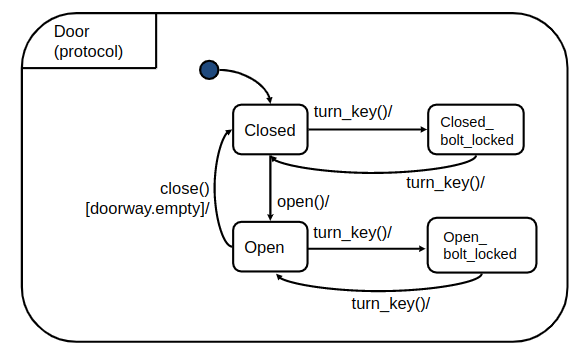
\includegraphics[scale=0.35]{img/exempleProtoStateMachine.png}
\end{wrapfigure}

\vspace{0.2cm}

\textrm{Il n'est pas pertinent de s'intéresser aux états d'ouvertures de la porte (\textit{ex : fermée contre, entre ouverte, etc...}). Ces états ne sont pas pertinents dans la description du verrouillage/déverrouillage d'une porte. On retiendra donc simplement les états ouverts et fermés.}

\vspace{0.2cm}

\textrm{De plus, on remarquera que le diagramme possède des changements d'états. Il s'agit d'action faisant transiter l'objet d'un état à un autre(\textit{ex : close()}). Mais il y a également des gardes qui conditionnent le changement d'état (\textit{ex : [doorway.empty]}).}


\vspace{1.5cm}

Il y a une volonté de simplifier les transitions en les rendant instantanées. Les postconditions sont généralement laissées à la définition de l'élément.

\subsubsection{Les évènements}

Parmi les évènements pouvant faire changer l'état d'un objet, voici les plus récurrents :

\begin{itemize}
    \item \textbf{Call Event} : Appel de fonction synchrone d'un objet. \textit{(ex : open(), close(), etc)}
    \item \textbf{Signal Event} : Réception d'un signal asynchrone d'un objet. \textit{(ex : onAlarmDetection, etc)}
    \item \textbf{Change Event} : Réception d'un signal asynchrone correspondant à une condition préalable \textit{(ex : when (a>0), when (isOpen), ...)}
    \item \textbf{Time Rvent} : Déclenchement d'un état après un certain temps ou à partir d'une certaine heure.
\end{itemize}

\vspace{0.2cm}

Le gros avantage de cette approche est qu'elle permet la méthode \textit{Divide and Conquer} en permettant de raisonner à un niveau d'état plutôt qu'avec un seul objet possédant des propriétés différentes.

Mais le schéma obtenu étant simplifié, il existe généralement des possibilités qui n'y sont pas reprises. Par exemple, dans l'illustration avec le verrouillage de porte, que se passe-t-il si on claque la porte ? Rien ne l'indique dans le schéma. Il faut alors indiquer ce qu'il se passe lorsqu'un évènement inattendu se produit :

\begin{center}
    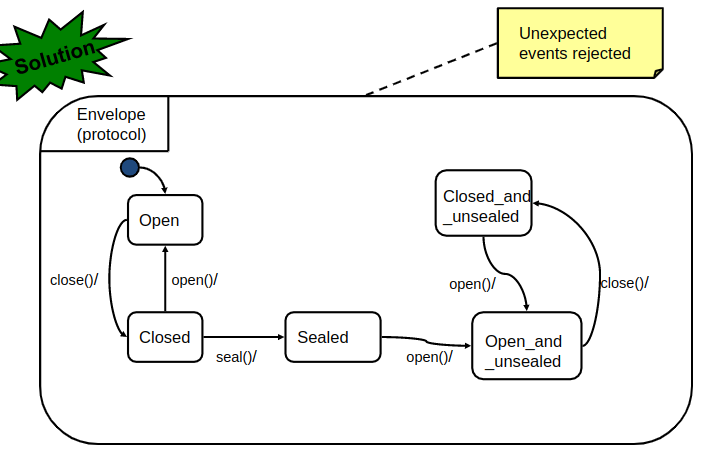
\includegraphics[scale=0.35]{img/exempleUnexpectedEvent.png}    
\end{center}

\subsection{Machine orthogonale à états}

Permet de répondre à la multiplication des états générée par les machines à état protocolaire, tout en réalisant en même temps une séparation des préoccupations.

% Picture wrapping
% use :             [lines]{align}{size}
\begin{wrapfigure}[8]{l}{0cm}
    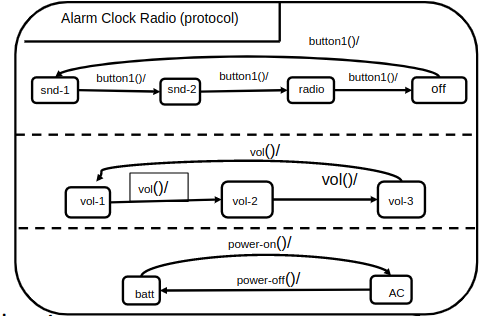
\includegraphics[scale=0.35]{img/exempleOrthogonalMachine.png}
\end{wrapfigure}

L'exemple ci-contre permet de représenter en 9 nœuds une machine à état qui, de façon classique, en aurait nécessité 24. On sépare alors les états qui peuvent l'être : on n'a pas besoin de gérer les changements d'états de l'alarme lorsque l'on règle le son.

On a également la possibilité de poser des gardes, comme avec la machine à état classique. Mais on peut ici poser des contraintes sur les états des nœuds parallèles. On peut donc empêcher l'activation d'un état tant qu'un autre état n'a pas été atteint dans un des schémas parallèles.

\vspace{0.7cm}

\subsection{Machine hiérarchique à états}

Pour éviter d'avoir une seule grosse machine à état illisible, on peut inclure des \textit{sous-schémas} qui permettent d'alléger le schéma principal.

% Picture wrapping
% use :             [lines]{align}{size}
\begin{wrapfigure}[2]{l}{0cm}
    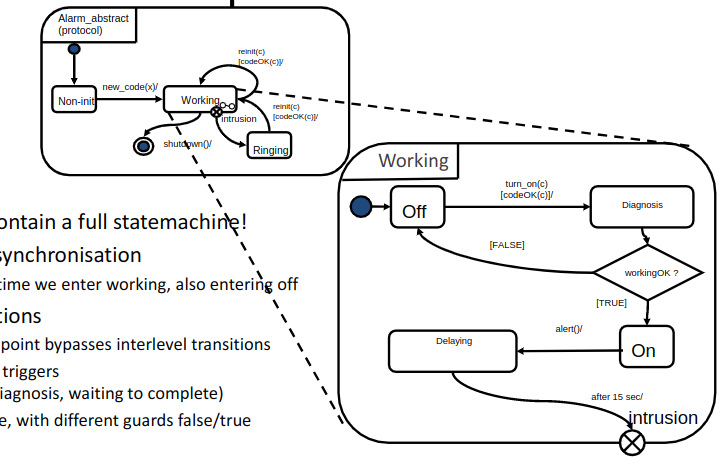
\includegraphics[scale=0.35]{img/exempleHierarchicalMachine.png}
\end{wrapfigure}

Un simple composant peut alors cacher une machine à états. On voit ici l'introduction du nœud de test, sous forme de losange.

\vspace{6cm}

\subsection{Transitions spéciales}

\subsubsection{Fork/Join}

% Picture wrapping
% use :             [lines]{align}{size}
\begin{wrapfigure}[2]{l}{0cm}
    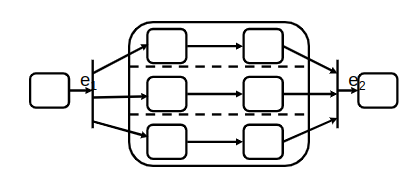
\includegraphics[scale=0.35]{img/fork.png}
\end{wrapfigure}

Explose ou fusionne des transitions pour les distribuer ou les récupérer sur différents états orthogonaux.

\vspace{2cm}

\subsubsection{Choix}

% Picture wrapping
% use :             [lines]{align}{size}
\begin{wrapfigure}[2]{r}{0cm}
    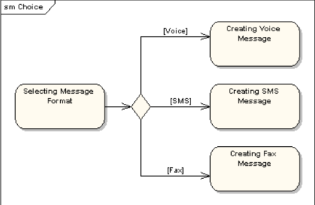
\includegraphics[scale=0.35]{img/choice.png}
\end{wrapfigure}

Permet de pauser une condition sur une transition, et de dispatcher la transition en question en fonction de l'évaluation de la condition.

\vspace{2cm}

\subsubsection{Jonction}

% Picture wrapping
% use :             [lines]{align}{size}
\begin{wrapfigure}[2]{l}{0cm}
    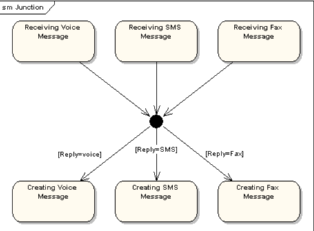
\includegraphics[scale=0.35]{img/junction.png}
\end{wrapfigure}

Permet d'effectuer un choix statique entre les possibles valeurs de sorties.


\end{document}
